The scheduling semantics can often be directly modeled in the AADL AGREE annex. At the component level, this requires introducing two Boolean variables \emph{dispatch} and \emph{complete}, augmenting the original \emph{assumptions} and \emph{guarantees} with \emph{dispatch} and \emph{complete}, respectively, and adding additional \emph{guarantees} to enforce the output freeze rule. We often omit the assumptions of frozen inputs, as they are trivially satisfied by the schedule definition, the output freeze rule, and the system-level assumptions.

\begin{figure}[t!]
\centering
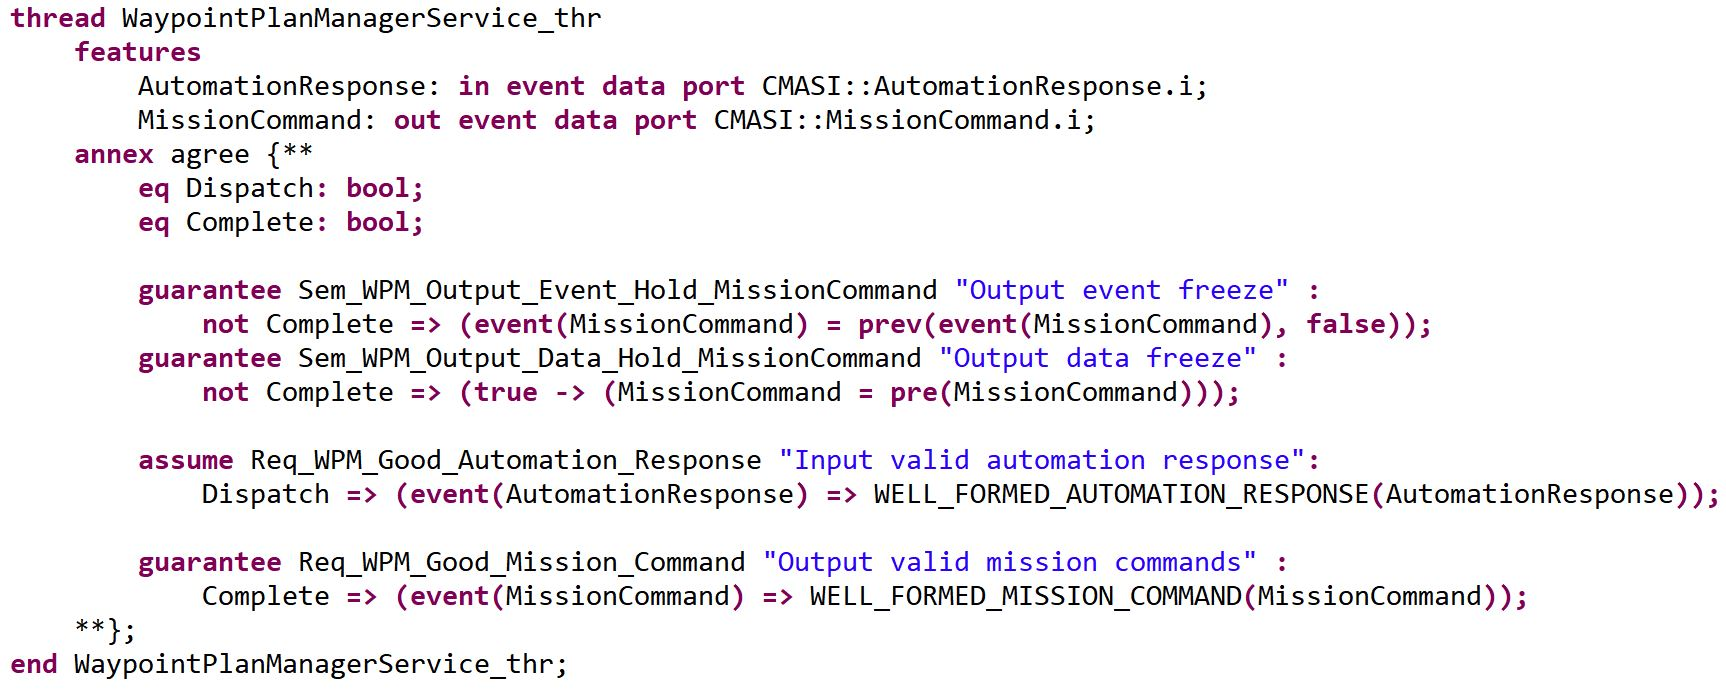
\includegraphics[width=130mm]{wpmAGREE3.jpg}
\caption{Modeling of Scheduling Semantics in AGREE\label{wpmAGREE}}
\end{figure}

Figure \ref{wpmAGREE} shows a simplified AADL model originally developed on the DARPA CASE program. The first two \emph{guarantees} are added to freeze the outputs between completions. The original contract (the assumption and the third \emph{guarantee}) are augmented with \emph{dispatch} and \emph{complete}.
In practice, we find that direct modeling is helpful to clarify the semantics with users. However, in general it could be a complex task, particularly if the contracts depend on past history. We rely on the Lustre backend model to handle the general case.

At the system-level, we use a circular counter to model a cyclic schedule in AGREE. 
The counter updates at every instant. Once it reaches the limit, it resets to one at the next instant.
We set the limit to the period of the schedule. 
%The counter is a direct encoding of schedule $\phi$ defined previously.
Based on the current count, the counter triggers a corresponding scheduling event.
Figure \ref{schedule} shows an AGREE model of the schedule $(ABACD)$.

\begin{figure}[t!]
\centering
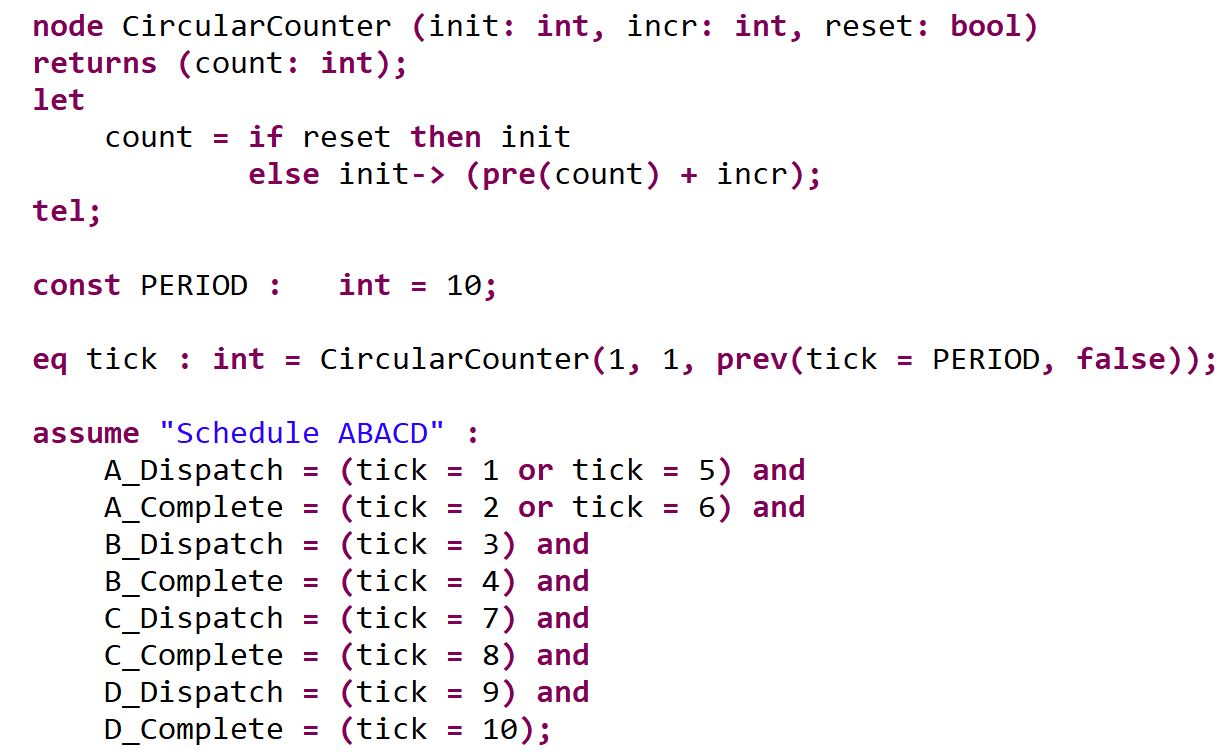
\includegraphics[width=80mm]{schedule.jpg}
\caption{Modeling Schedule with Circular Counter in AGREE\label{schedule}}
\end{figure}

%An AGREE model of the schedule $(ABACD)^*$ used in the example is shown in code~\ref{schedule_model}

%\begin{lstlisting}[language=c,frame=single,caption=An AGREE model of a schedule,label=schedule_model]
%node CircularCounter (init: int, incr: int, reset: bool)	
%returns (count: int);
%let
%	count = if reset then init
%		else init-> (pre(count) + incr);
%tel;
%				
%eq tick : int = CircularCounter(1,1,prev(tick=10,false));
%
%assume "Schedule ABACD" :
%	A_dispatch = (tick = 1 or tick = 5) and
%	A_complete = (tick = 2 or tick = 6) and					
%	B_dispatch = (tick = 3) and	
%	B_complete = (tick = 4) and
%	C_dispatch = (tick = 7) and
%	C_complete = (tick = 8) and	
%	D_dispatch = (tick = 9) and
%	D_complete = (tick = 10);			
%\end{lstlisting}	

